\documentclass[spec, och, otchet, hidelinks]{SCWorks}
% параметр - тип обучения - одно из значений:
%    spec     - специальность
%    bachelor - бакалавриат (по умолчанию)
%    master   - магистратура
% параметр - форма обучения - одно из значений:
%    och   - очное (по умолчанию)
%    zaoch - заочное
% параметр - тип работы - одно из значений:
%    otchet
%    referat    - реферат
%    coursework - курсовая работа (по умолчанию)
%    diploma    - дипломная работа
%    pract      - отчет по практике
%    pract      - отчет о научно-исследовательской работе
%    autoref    - автореферат выпускной работы
%    assignment - задание на выпускную квалификационную работу
%    review     - отзыв руководителя
%    critique   - рецензия на выпускную работу
% параметр - включение шрифта
%    times    - включение шрифта Times New Roman (если установлен)
%               по умолчанию выключен
\usepackage[T2A]{fontenc}
\usepackage[utf8]{inputenc}
\usepackage{graphicx}

\usepackage[sort,compress]{cite}
\usepackage{amsmath}
\usepackage{amssymb}
\usepackage{amsthm}
\usepackage{fancyvrb}
\usepackage{longtable}
\usepackage{array}
\usepackage[english,russian]{babel}
\usepackage{minted}
% Используется автором репозитория
%\usemintedstyle{xcode}
% Этот пакет включает в себя аналогичный Times New Roman шрифт.
% Необходим для успешной компиляции для UNIX-систем ввиду отсутствия TNR в нем.
% Можно использовать и для Windows.
\usepackage{tempora}


\usepackage[colorlinks=false]{hyperref}

\graphicspath{{figures/}}

\newcommand{\eqdef}{\stackrel {\rm def}{=}}

\usepackage{stackengine}
\newcommand\xrowht[2][0]{\addstackgap[.5\dimexpr#2\relax]{\vphantom{#1}}}

\newtheorem{lem}{Лемма}

% % При использовании biblatex вместо bibtex
%\usepackage[style=gost-numeric]{biblatex}
%\addbibresource{thesis.bib}

\begin{document}

% Кафедра (в родительном падеже)
\chair{математической кибернетики и компьютерных наук}

% Тема работы
\title{Цифроаналоговый преобразователь}

% Курс
\course{3}

% Группа
\group{331}

% Факультет (в родительном падеже) (по умолчанию "факультета КНиИТ")
%\department{факультета КНиИТ}

% Специальность/направление код - наименование
%\napravlenie{02.03.02 "--- Фундаментальная информатика и информационные технологии}
%\napravlenie{02.03.01 "--- Математическое обеспечение и администрирование информационных систем}
%\napravlenie{09.03.01 "--- Информатика и вычислительная техника}
%\napravlenie{09.03.04 "--- Программная инженерия}
\napravlenie{10.05.01 "--- Компьютерная безопасность}

% Для студентки. Для работы студента следующая команда не нужна.
%\studenttitle{Студентки}

% Фамилия, имя, отчество в родительном падеже
\author{Бородина Артёма Горовича}

% Заведующий кафедрой
\chtitle{доцент, к.\,ф.-м.\,н.} % степень, звание
\chname{С.\,В.\,Миронов}

%Научный руководитель (для реферата преподаватель проверяющий работу)
\satitle{аспирант}%, к.\,ф.-м.\,н.} %должность, степень, звание
\saname{А.\,А.\,Мартышкин}

% Руководитель практики от организации (только для практики,
% для остальных типов работ не используется)
\patitle{к.\,ф.-м.\,н., доцент}
\paname{Д.\,Ю.\,Петров}

% Семестр (только для практики, для остальных
% типов работ не используется)
\term{2}

% Наименование практики (только для практики, для остальных
% типов работ не используется)
\practtype{учебная}

% Продолжительность практики (количество недель) (только для практики,
% для остальных типов работ не используется)
\duration{2}

% Даты начала и окончания практики (только для практики, для остальных
% типов работ не используется)
\practStart{01.07.2016}
\practFinish{14.07.2016}

% Год выполнения отчета
\date{2022}

\maketitle

% Включение нумерации рисунков, формул и таблиц по разделам
% (по умолчанию - нумерация сквозная)
% (допускается оба вида нумерации)
%\secNumbering


\tableofcontents

\intro

Целью данной работы служит ознакомление с принципом работы интегрального цифроаналогового преобразователя, а также его испытание.

\newpage

\section*{Задание 1.}
\addcontentsline{toc}{section}{Задание 1}

Запустить лабораторный комплекс Labworks и среду МS10. Открыть файл \textbf{35.3.ms10}, размещенный в папке \textbf{Circuit Design Suitе 10.0} среды 
МS10, или собрать на рабочем поле среды MS10 схему для испытания интегрального \textit{цифроаналогового преобразователя} и установить в диалоговых 
окнах компонентов их параметры или режимы работы. \textbf{Скопировать} схему в отчет.

\begin{figure}[h]
	\center{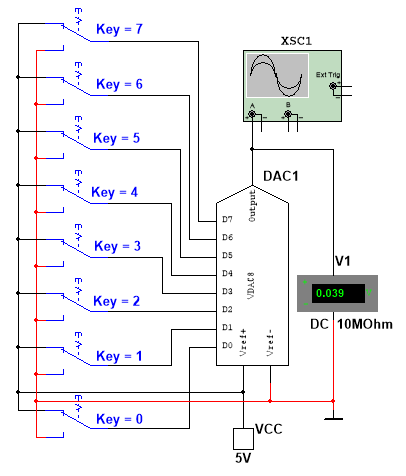
\includegraphics{scheme_task_one.png}}
	\caption{Схема интегрального цифроаналогового преобразователя.}
\end{figure}

\newpage

\section*{Задание 2.}
\addcontentsline{toc}{section}{Задание 2}

\textbf{Получить} на экране осциллографа \textbf{XSC1} ступенчатое выходное напряжение ЦАП. Для этого нужно вначале замкнуть переключатель \textbf{0}, 
то есть подать напряжение 5 В на вход \textbf{D0} ЦАП, и запустить программу моделирования. На выходе ЦАП формируется напряжение, равное ЗМР. Затем во 
время остановок моделирования замыкать поочередно переключатели \textbf{1, 2}, $ \dots $, \textbf{7}, подавая входные десятичные комбинации 3, 7, 
$ \dots $, 255 на входы \textbf{D0}, $\dots$, \textbf{D7} ЦАП.

\begin{figure}[h]
	\center{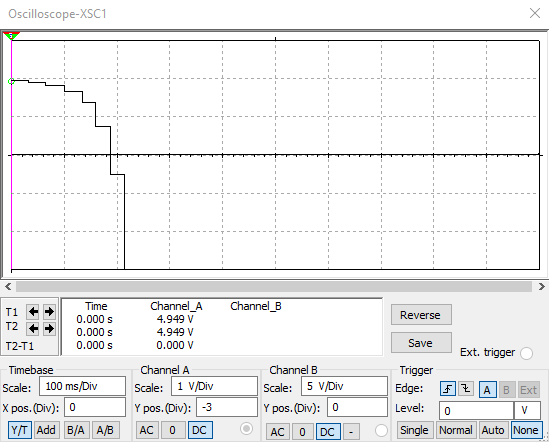
\includegraphics{step_voltage.png}}
	\caption{Ступенчатое выходное напряжение ЦАП.}
\end{figure}

\newpage

\textbf{Повторить} эксперимент, подавая на входы ЦАП сформированые с помощью переключателей шестнадцатеричные коды от 0 до FF $(255_{10})$ через шаг 
$10_{16} (16_{10})$ и занося в табл. 1 показания вольтметра \textbf{V1} (значения выходного напряжения $ u_\text{вых} $ ЦАП) при напряжении источника 
\textbf{VCC} $ u_\text{o} $ = 5 В. \textbf{Найти} частичные и усредненное значения ступени, частичные и усредненное значения МЗР. \textbf{Построить} 
график $ u_\text{вых}(N) $, выбрав соответствующие масштабы для напряжений и входных десятичных чисел $N$, откладываемых по осям координат.

\begin{table}[h!]
	\centering
	\captionsetup{justification=centering}
	\begin{tabular}{|c|c|c|c|c|}
		\hline\xrowht[()]{10pt}
		№ п/п & $N$ & $ u_\text{вых.} $, В & $ u_\text{вых.1} - u_\text{вых.2},$ В & $(u_\text{вых.1} - u_\text{вых.2})/16,$ В \\
		\hline\xrowht[()]{10pt}
		1    &     0   &   0   &   0   &  -- \\
		\hline\xrowht[()]{10pt}
		2    &    15   &   0.312   &   4.688   &  0.293 \\
		\hline\xrowht[()]{10pt}
		3    &    31   &   0.623   &   4.377   &  0.27356 \\
		\hline\xrowht[()]{10pt}
		4    &    47   &   0.935   &   4.065   &  0.25406 \\
		\hline\xrowht[()]{10pt}
		5    &    63    &  1.247   &   3.753   &  0.23456 \\
		\hline\xrowht[()]{10pt}
		6    &    79   &   1.559   &   3.441   &  0.21506 \\
		\hline\xrowht[()]{10pt}
		7    &    95   &   1.87    &   3.13    &  0.19562 \\
		\hline\xrowht[()]{10pt}
		8    &   111   &   2.182   &   2.818   &  0.17612 \\
		\hline\xrowht[()]{10pt}
		9    &   127   &   2.494   &   2.506   &  0.15662 \\
		\hline\xrowht[()]{10pt}
		10    &  143   &   2.805   &   2.195   &  0.13718 \\
		\hline\xrowht[()]{10pt}
		11    &  159   &   3.117   &   1.883   &  0.11768 \\
		\hline\xrowht[()]{10pt}
		12    &  175   &   3.429   &   1.571   &  0.09818 \\
		\hline\xrowht[()]{10pt}
		13    &  191   &   3.741   &   1.259   &  0.07868 \\
		\hline\xrowht[()]{10pt}
		14    &  207   &   4.052   &   0.948   &  0.05925 \\
		\hline\xrowht[()]{10pt}
		15    &  223   &   4.364   &   0.636   &  0.03975 \\
		\hline\xrowht[()]{10pt}
		16    &  239   &   4.676   &   0.334   &  0.02087 \\
		\hline\xrowht[()]{10pt}
		17    &  255   &   4.988   &   0.12    &  0.0075 \\
		\hline
	\end{tabular}
	\caption{Значения выходного напряжения $u_\text{вых.}$ ЦАП.}
\end{table}
В этой таблице $N$ - входной десятичный код, $u_\text{вых.}$ - выходное напряжение, $u_\text{вых.1} - u_\text{вых.2}$ - напряжение ступени, 
$(u_\text{вых.1} - u_\text{вых.2})/16$ - значение младшего рязряда МЗР.

\newpage

\par Построим график $ u_\text{вых.} (N) $. По оси $x$ располагаются входные десятичные коды, а по оси $y$ - получающиеся значения выходного напряжения.

\begin{figure}[h]
	\center{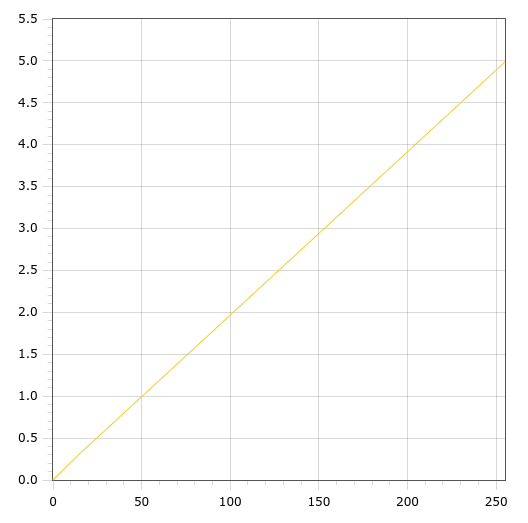
\includegraphics[scale=0.7]{plot.png}}
	\caption{График $u_\text{вых.}(N)$.}
\end{figure}

\newpage

\section*{Задание 3.}
\addcontentsline{toc}{section}{Задание 3}

Открыть файл \textbf{35.4.ms10}, размещенный в папке \textbf{Circuit Design Suitе 10.0} среды МS10, или собрать на рабочем поле среды MS10 схему для 
испытания \textit{цифроаналогового преобразователя} и установить в диалоговых окнах компонентов их параметры или режимы работы. Скопировать схему в 
отчет.

\begin{figure}[h]
	\center{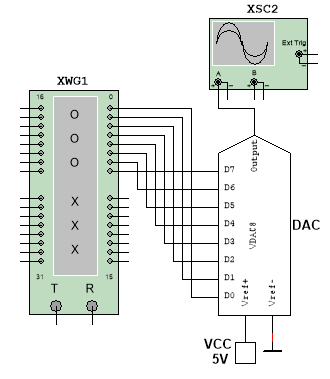
\includegraphics{scheme_task_three.png}}
	\caption{Схема для испытания цифроаналогового преобразователя.}
\end{figure}

\newpage

\textbf{Провести} моделирование ЦАП, запрограммировав генератор \textbf{XWG1} (частота генерации сигналов $ f_\text{г} = $ 1 кГц) на возрастание и 
убывание шестнадцатеричных чисел от 0 до FF $(255_{10})$ при шаге $10_{16}$ ($16_{10}$).

\begin{figure}[h]
	\center{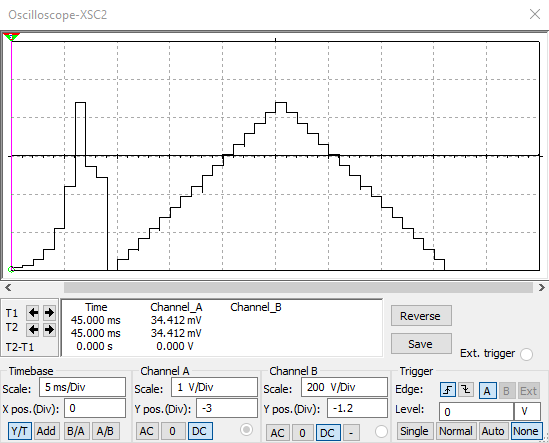
\includegraphics[scale=0.77]{pyramid_voltage.png}}
	\caption{Моделирование ЦАП на возрастающих и убывающих шестнадцатиричных числах.}
\end{figure}

\textbf{Установить} напряжение $ u_0 = $ 10 В источника \textbf{VCC} и \textbf{повторить} моделирование ЦАП при опорном напряжении 10 В. 

\begin{figure}[h!]
	\center{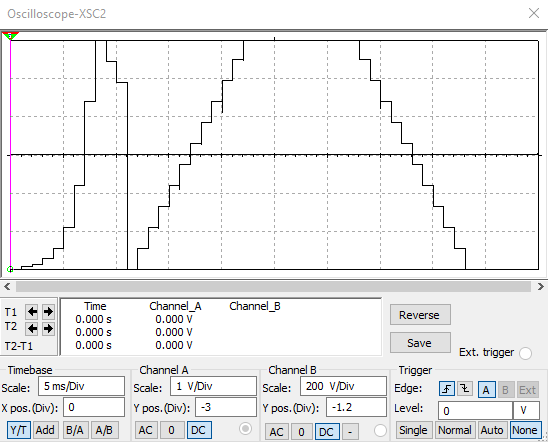
\includegraphics[scale=0.77]{voltage_ten.png}}
	\caption{График $u_\text{вых.}(N)$ при $u_0$ = 10.}
\end{figure}

\newpage

\section*{Тестовые задания.}
\addcontentsline{toc}{section}{Тестовые задания}

\par 1. Укажите \textbf{назначение} ЦАП: \textbf{для преобразования цифрового кода $N$ в пропорциональное аналоговое значение напряжения $u(N)$};

\par 2. Укажите, какая \textbf{структура резистивных матриц} ЦАП имеет преимущество при изготовлении преобразователя посредством интегральной технологии: 
\textbf{матрица $R - 2R$}.

\par 3. Определите понятие «\textbf{абсолютная разрешающая способность}» ЦАП: \textbf{это среднее значение минимального изменения сигнала на выходе ЦАП, 
обусловленное увеличением или уменьшением его кода на единицу};

\par 4. Укажите, для чего выбирают опорное напряжение \textbf{двуполярным}: \textbf{чтобы получать на выходе двуполярное напряжение $\pm u_\text{вых}$ при 
различных входных кодах};

\par 5. Укажите \textbf{перспективы развития} ЦАП: \textbf{повышение быстродействия ключей и уменьшение времени установки ОУ; применение стабилизированных источников опорного напряжения}.

\conclusion

В ходе данной лабораторной работы мы ознакомились с принципом работы интегрального цифроаналогового преобразователя, а также испытали его на практике.

\end{document}